
\documentclass[letterpaper,12pt]{article}
\usepackage{tabularx} 
\usepackage{amsmath}  
\usepackage{amsthm}
\usepackage{amsfonts}
\usepackage{graphicx} 
\usepackage[margin=1in,letterpaper]{geometry} 
\usepackage{cite} 
\usepackage{graphicx} 
\usepackage[spanish]{babel}
\usepackage[export]{adjustbox}
\usepackage{wrapfig}
\usepackage[final]{hyperref} 
\usepackage[utf8]{inputenc}
\usepackage{float}
\usepackage{helvet}
\usepackage{pdfpages}
\renewcommand{\familydefault}{\sfdefault}
\hypersetup{
	colorlinks=true,      
	linkcolor=blue,       
	citecolor=blue,       
	filecolor=magenta,    
	urlcolor=blue         
}
\graphicspath{ {d:/proyectos/universidad/LaHoraDelCodigo/Planificacion/} }



\title{Propuesta de Organización para el Evento \\ \texttt{\textbf{HoraDelCódigo}} }
\author{Gonzalo Fernández C. \\ \texttt{gonzalo.fernandezc@sansano.usm.cl} }
\date{\today\\Revisión 1.1}

\usepackage{titling}
\setlength{\droptitle}{0.6in}
 
\begin{document}

\begin{titlepage}

\begin{figure}

\includegraphics[width=0.4\linewidth]{logou} 
\hspace{\fill}

\includegraphics[width=0.08\linewidth]{logo} 
\end{figure}

\maketitle

\end{titlepage}


\section{Historial de Cambios}

\begin{center}
\begin{tabular}{|c|c|c|l|}
\hline
Versión & Fecha & Autor & Comentario \\
\hline \hline
1.0 & 17/01/2018 & Gonzalo F. & Primera versión del documento \\ \hline
1.1 & 04/03/2018 & Gonzalo F. & Correciones sugeridas por el profesor Pedro Godoy \\ \hline
\end{tabular}
\end{center}

\section{Introducción}

El presente documento pretende formalizar una propuesta de organización con el fin de realizar una \texttt{HoraDelCódigo} en la \texttt{Universidad Técnica Federico Santa María - Campus San Joaquín}. En este se tratarán temas relacionados con los tutores, participantes, los procesos de inscripción e invitación, tiempos, talleres, costos, recursos necesarios, entre otros. Al no ser esta una propuesta definitiva, el documento está abierto a modificaciones posteriores con el fin de lograr organizar de mejor forma la realización de este evento.\\

La \texttt{HoraDelCódigo} es un evento en que se brinda una introducción a niños y niñas para entender la programación computacional de manera fácil y entretenida, en esta, se realizan talleres especialmente desarrolladas para que durante 1 hora niños y niñas puedan adentrarse en el mundo de las ciencias de la computación sin necesidad de que estos tengan alguna experiencia previa. Tanto es el impacto de este evento que anualmente se realizan Horas Del Código en más de 180 países alrededor del mundo llegando a decenas de millones de estudiantes.\\

Los talleres a desarrollar durante esta \texttt{HoraDelCódigo} son extraídos del sitio web oficial \href{https://hourofcode.com/us/learn}{https://hourofcode.com/us/learn} y guiados por alumnos de la universidad los cuales han repasado tanto los talleres como el material docente que estos proveen. Estos contemplan una duración de a lo más 1 hora y se realizarán en paralelo el día del evento.

\vfill

\section{Tutores}

El ideal para la realización de estos talleres es contar con la participación de a lo más 2 tutores por actividad. Actualmente, los siguientes alumnos se han ofrecido voluntariamente a participar como tutores en esta actividad guiándo a los asistentes en la realización de alguno de los talleres ofrecidos por \texttt{\textbf{HoraDelCódigo}}:

\begin{itemize}
    \item Gonzalo Fernández C. -- \texttt{gonzalo.fernandezc@sansano.usm.cl} 
    \item Martin Crisostomo B. -- \texttt{martin.crisostomo@sansano.usm.cl} 
    \item Fabian Riquelme M. -- \texttt{fabian.riquelme@sansano.usm.cl}
    \item Christian Muñoz I. -- \texttt{christian.munozi@sansano.usm.cl}
    \item Sebastian Alvarado A. -- \texttt{sebastian.alvaradoa@sansano.usm.cl}
\end{itemize}

\section{Participantes}

El público objetivo para este evento son alumnos que estén cursando entre 1er y 4to año de enseñanza media, distribuídos en 10 alumnos por taller, dado que para esta ocasión se realizarán 5 talleres, el total de participantes no debería exceder los 50 alumnos. Para llevar esto a cabo, se espera contar con el apoyo del área de admisión de la universidad.

\section{Talleres}

Los talleres fueron elegidos desde el \texttt{\href{https://hourofcode.com/es/learn}{Sitio Oficial}} de \texttt{HoraDelCódigo} por parte de los Tutores encargados de realizar cada uno. Cada taller requiere de 1 laboratorio con equipos para poder realizarse, estos se detallan a continuación:

\subsection{Mazmorra de Kithgar}

 Juego en el cual se deben cumplir los objetivos usando programación en Python, aprendiendo Python a medida que se van avanzando en los niveles.

\begin{itemize}
    \item Tutores: Martin Crisostomo B. -- Pendiente.
    \item Laboratorio: Lab 1 (B-03X).
    \item Requerimientos: PC Linux/Windows con Navegador Web (Google Chrome ó Firefox).
    \item Sitio Web: \href{https://codecombat.com/play/dungeon?hour_of_code=true}{https://codecombat.com/}
\end{itemize}

\subsection{Evasión de Asteroides}

Diseña un clásico videojuego de naves de forma simple y rápida. No necesitas conocimientos en programación, sólo tener creatividad y hacer uso de la programación \texttt{Drag \& Drop}, a la vez podrás ver y editar el codigo resultante de tu juego para personalizarlo y lograr los objetivos solicitados. 

\begin{itemize}
    \item Tutores: Fabian Riquelme M. -- Pendiente.
    \item Laboratorio: Lab 2 (B-03X).
    \item Requerimientos: PC Linux/Windows con Navegador Web (Google Chrome ó Firefox).
    \item Sitio Web: \href{https://www.codesters.com/curriculum/hour-of-code-2017/Evasi%25C3%25B3n+de+Asteroides/25/}{https://www.codesters.com/}

\end{itemize}

\subsection{3 Retos Rápidos y Divertidos}

Este taller consta de 3 talleres: 

\begin{itemize}
  \item[--]\textbf{Anima tu nombre}: Se crea una animación interactiva del nombre de uno utilizando JavaScript sin necesidad de saber algo de programación ya que allí se enseñarán los conceptos más básicos, tales como: Strings, Booleanos, Arrays, entre otros... Allí se podrá personalizar utilizando distintos colores para personalizar el nombre a gusto, al igual que las formas geométricas que se usarán para animar el nombre.
  \item[--] \textbf{Sobre ti}: Se enseña paso a paso los aspectos más generales sobre la creación de una página web utilizando HTML5 y CSS para darle estilo a la página con el fin de crear una página autobiográfica.
  \item[--] \textbf{Sol, Tierra y Código}: Utilizando solo HTML5 y CSS se crea un sistema planetario compuesto del Sol y la Tierra, utilizando imágenes de internet y estilos con CSS. La idea final es lograr poder crear un propio sistema planetario más complejo una vez terminada la actividad empleando más planetas, órbitas y demases.
\end{itemize}

\begin{itemize}
  \item Tutores: Sebastian Alvarado A. -- Pendiente.
  \item Laboratorio: Lab 3 (B-03X).
  \item Requerimientos: PC Linux/Windows con Navegador Web (Google Chrome ó Firefox).
  \item Sitio Web: 
    \begin{itemize}
      \item \href{https://www.codecademy.com/courses/animate-your-name/0/1}{Tu Nombre Animado.}
      \item \href{https://www.codecademy.com/en/courses/web-beginner-en-3pc6w/0/1}{Tu Primer Sitio Web}
      \item \href{https://www.codecademy.com/courses/web-beginner-en-ymqg0/0/1}{Sol, Tierra y Código}
    \end{itemize}

\end{itemize}

\subsection{Minecraft: Viaje del héroe}

Guía a Steve ó Alex en una aventura a través del mundo de Minecraft usando Programación en bloques y tu creatividad.

\begin{itemize}
    \item Tutores: Gonzalo Fernández C. -- Pendiente.
    \item Laboratorio: LPA (B-03X).
    \item Requerimientos: PC Linux/Windows con Navegador Web (Google Chrome ó Firefox).
    \item Sitio Web: \href{https://studio.code.org/s/hero/stage/1/puzzle/1}{https://studio.code.org/}
\end{itemize}

\subsection{Diseños de Erizo}

En esta actividad, diseñada para programadores principiantes, los estudiantes usarán una plataforma de \texttt{Drag \& Drop} para comenzar a programar en Python de la forma correcta!. Primero, trabajarán algunas habilidades mediante la modificación y asignación de comandos para tu erizo, y entonces, programarán los comandos necesarios para hacer arte mediante algoritmos. 

\begin{itemize}
    \item Tutores: Christian Muñoz I. -- Pendiente.
    \item Laboratorio: Lab 2 (B-03X).
    \item Requerimientos: PC Linux/Windows con Navegador Web (Google Chrome ó Firefox).
    \item Sitio Web: \href{https://www.codesters.com/curriculum/hour-of-code-2017/Dise%25C3%25B1os+de+Erizo/23/}{https://www.codesters.com/}
\end{itemize}

\begin{figure}[H]
  \centering
    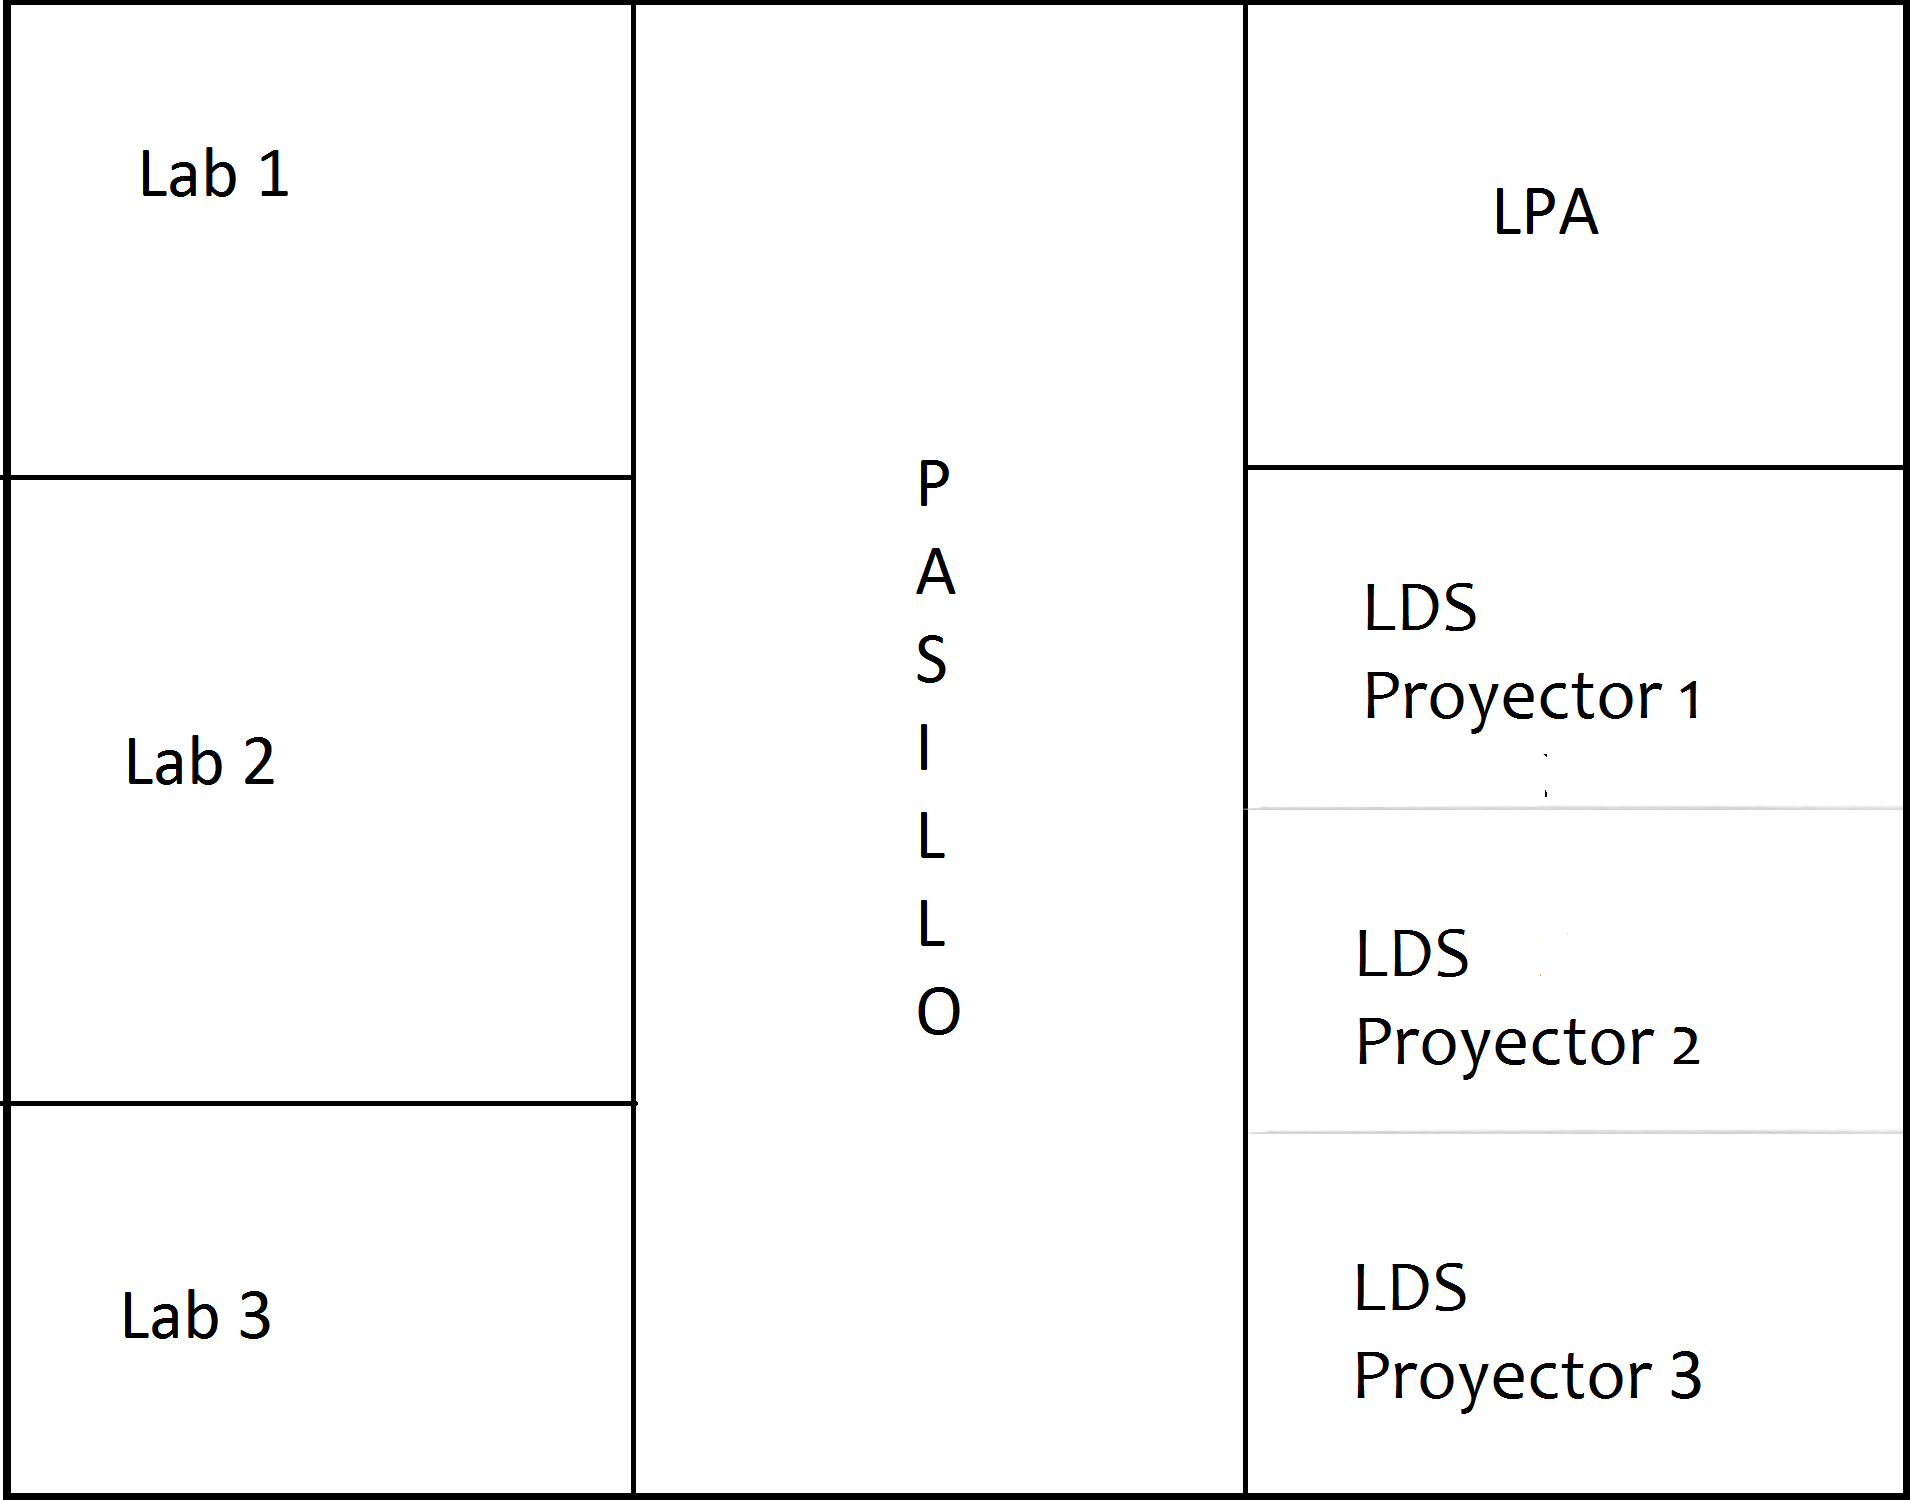
\includegraphics[width=0.5\textwidth]{salas}
  \caption{Distribución de los laboratorios para el evento.}
\end{figure}

\section{Horarios}

La fecha tentativa de realización de este evento es el día \textbf{Viernes 23 de Marzo}, en la siguiente tabla se detallan las actividades a realizar:

\begin{center}
\begin{tabular}{|c|c| p{11cm} |}
\hline
Actividad & Duración & Comentario \\
\hline \hline
Preparación & 9:30 -- 10:00 & Llegada de los Tutores y gente encargada de organizar el evento para preparar todo. \\ \hline
Acreditación & 10:00 -- 10:30 & Llegada de los participantes, presentación del evento. \\ \hline
\texttt{HoraDelCódigo} & 10:30 -- 12:30 & Distribución de los alumnos en los distintos laboratorios e inicio de talleres. \\ \hline
Colación & 12:30 -- 12:45 & Término de los talleres, se entregan colaciones a los participantes. \\ \hline
Despedida & 12:45 & Se entregan diplomas de participación, terminan las actividades. \\ \hline
\end{tabular}
\end{center}

\section{Costos}

Los costos de la realización de este evento serían:

\begin{center}
\begin{tabular}{|c|c|c| p{11cm} |}
\hline
Item & Cantidad & Precio & Comentario \\
\hline \hline
Poleras & 10 & ? & Poleras estampadas con el logo de la universidad, departamento de informática y HoraDelCódigo\\ \hline
Colaciones & 60 & ? & Colaciones para los participantes y monitores, falta determinar de qué estará compuesta. \\ \hline
Diplomas & 50 & ? & Impresión de diplomas de participación (diseño pendiente). \\ \hline
\end{tabular}
\end{center}

\vfill

\section{Diseños}

\subsection{Poleras}

\begin{figure}[H]
  \centering
    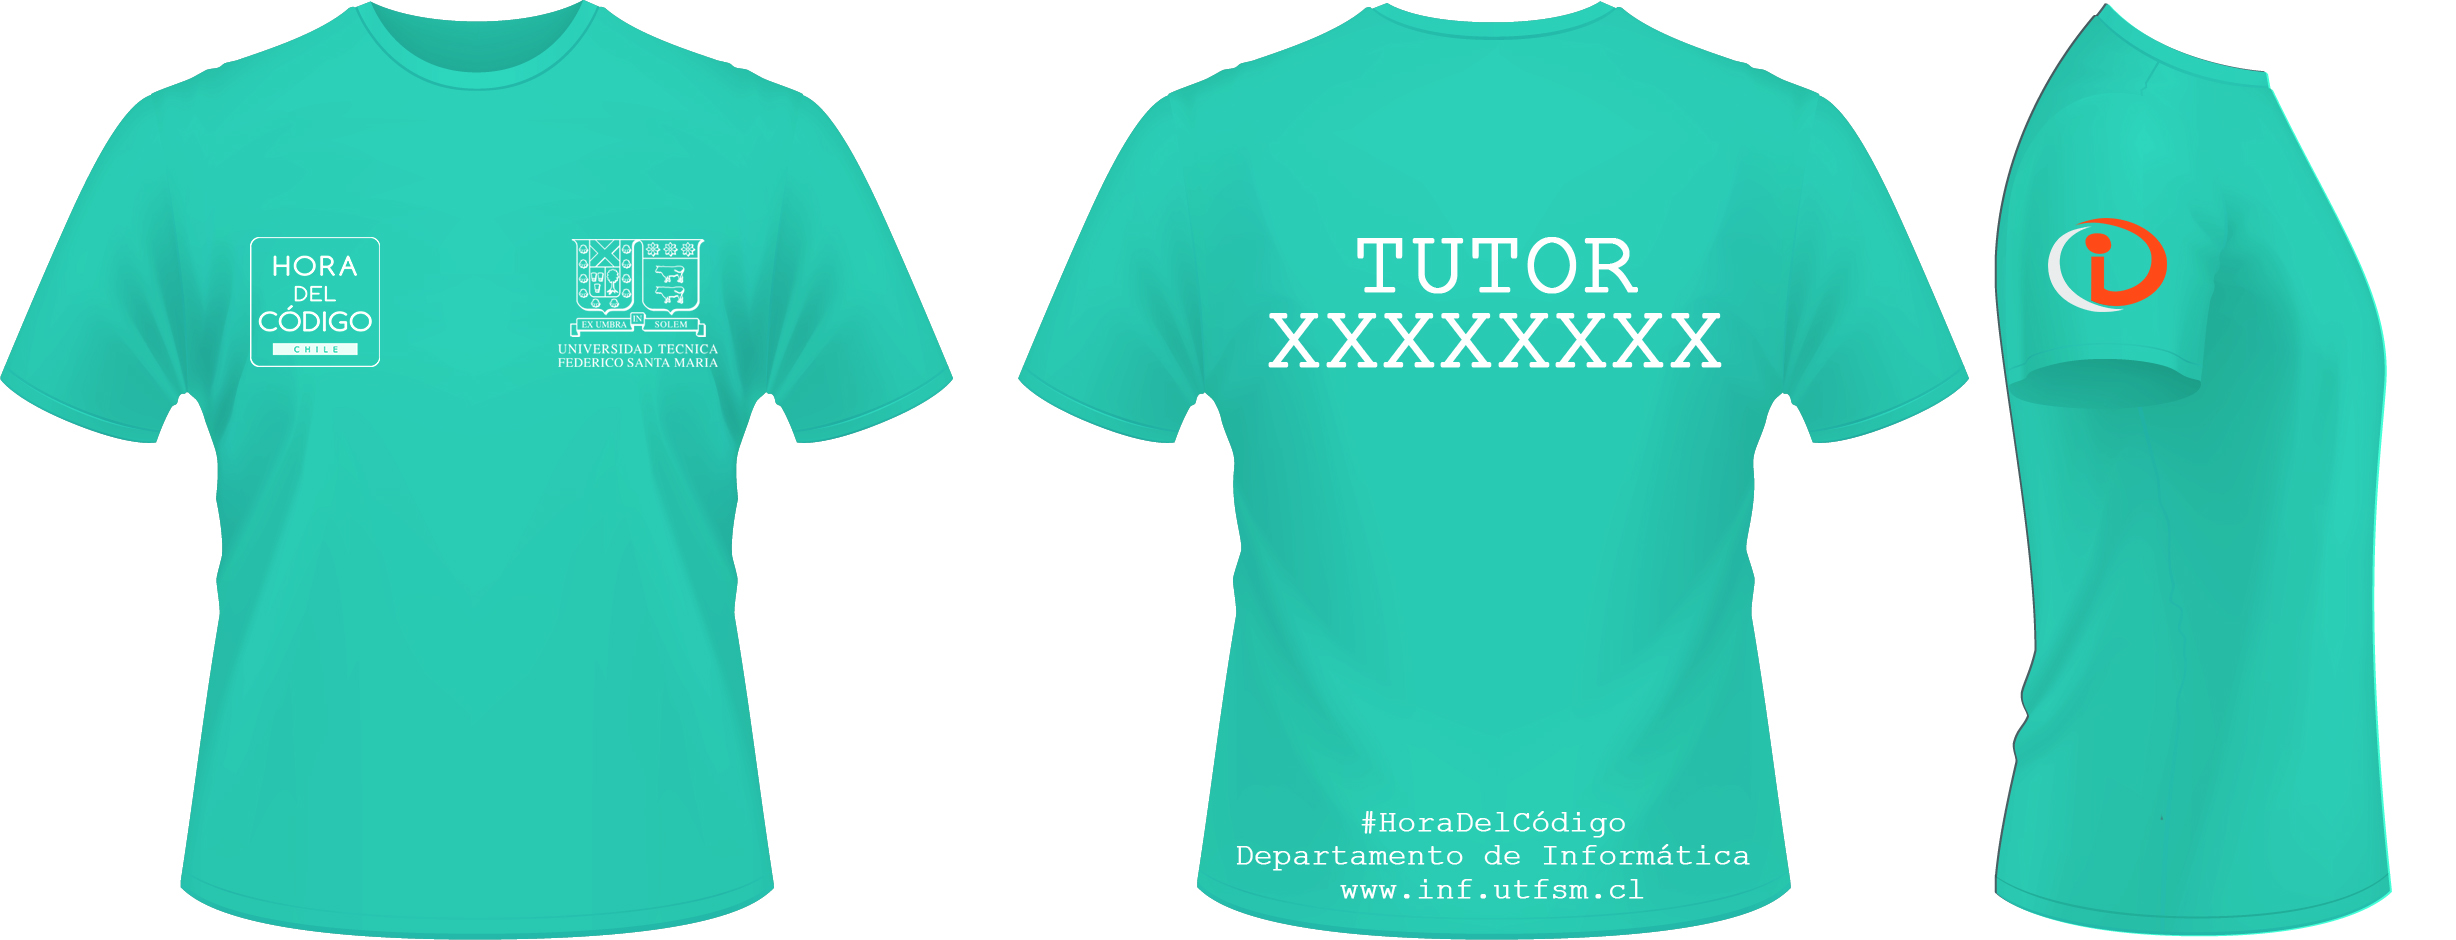
\includegraphics[width=1.0\textwidth]{poleras.jpg}
  \caption{Diseño para las poleras de los tutores.}
\end{figure}

\subsection{Diplomas}

\begin{figure}[H]
  \centering
    
\includegraphics[width=1.0\textwidth]{diploma.png}
  \caption{Diseño para los diplomas de los participantes.}
\end{figure}

\section{Pendientes}

A continuación se detallan temas pendientes a concretar dentro de esta propuesta de organización:

\begin{itemize}

  \item Determinar de qué estarán compuestas las colaciones.
  \item Encontrar 5 monitores más (En proceso).

\end{itemize}

\end{document}